\chapter{Agronegócio}
\par A agricultura é importante para o Brasil, é um setor que cresce de forma exponencial e alavanca a economia de inúmeros estados da federação. O agronegócio representou 21,4\% do \acrshort{pib} nacional em 2019, demonstrando o quão providencial é para o país. Já para o Tocantins, sua participação está abaixo da média nacional, pois o agronegócio está abaixo de 15\% da representação do \acrshort{pib} estadual. Nesta sessão do Boletim apresenta-se os seguintes dados da agricultura; Área de produção, colhida, produção de cereais e oleaginosas e o seu rendimento médio. Em outra parte analise-se os dados de abates de animais, produção de ovos de galinha e leite.
\par Nas páginas a seguir é apresentado os dados mais relevantes para o agronegócio estadual e para a conjuntura do semestre, sabe-se que uma análise total das cadeias produtivas da agricultura requerem estudos mais aprofundados. Aqui, iremos apresentar e analisar os dados de mais relevância por produção e participação no cenário econômico.

% \section{Produção}
\par O estado do Tocantins apresentou no primeiro semestre de 2020 uma produção  equivalente a 1.520.698 hectares. Dentre os 5 principais produtos plantados no estado, conforme a Figura \ref{fig:lavouras}, destaca-se as elevadas quantidades providas da cana-de-açúcar e soja, responsáveis por 38.2\% e 36.2\% do total produzido, seguido pelo milho como o terceiro produto mais cultivado no estado neste período correspondendo à 14.5\%. A produção de arroz e mandioca também ganha destaque ao representar um montante de 8.2\% e 3\% respectivamente, fechando assim o ranking dos cinco produtos com maior influência na agricultura tocantinense.

\begin{figure}[!h]
	\begin{subfigure}{\linewidth}
		\caption{Produção das principais lavouras}
		\subcap{Em milhões de toneladas. Estimativa anual de setembro}
		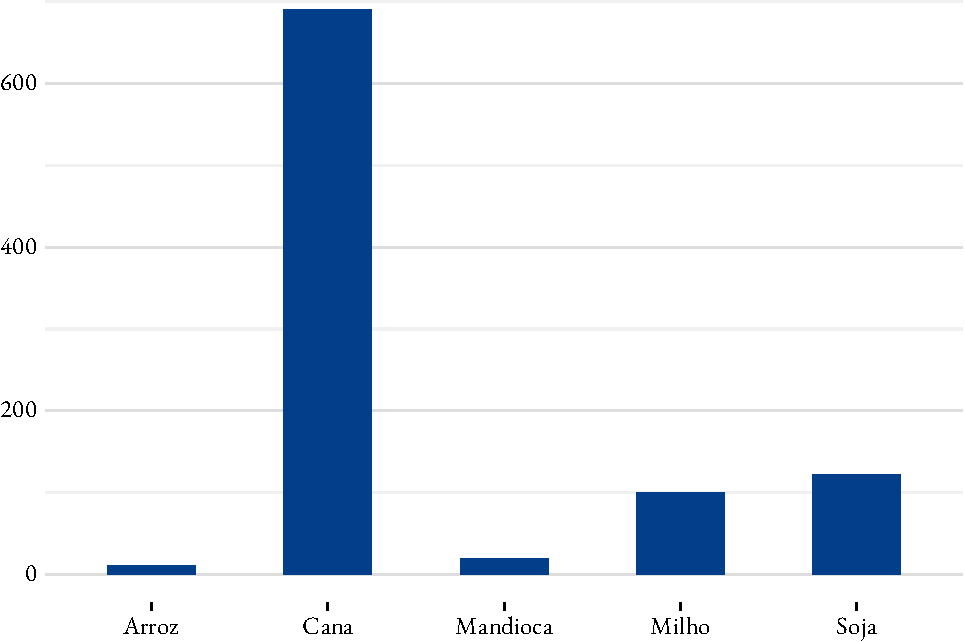
\includegraphics{fig/producao-1.pdf}
		\source{\acrshort{sidra}/\acrshort{ibge}}
		\label{fig:lavouras}
	\end{subfigure}
	\begin{subfigure}{\linewidth}
		\caption{Rendimento médio das lavouras}
		\subcap{Mil quilogramas por hectare. Estimativa anual de setembro}
		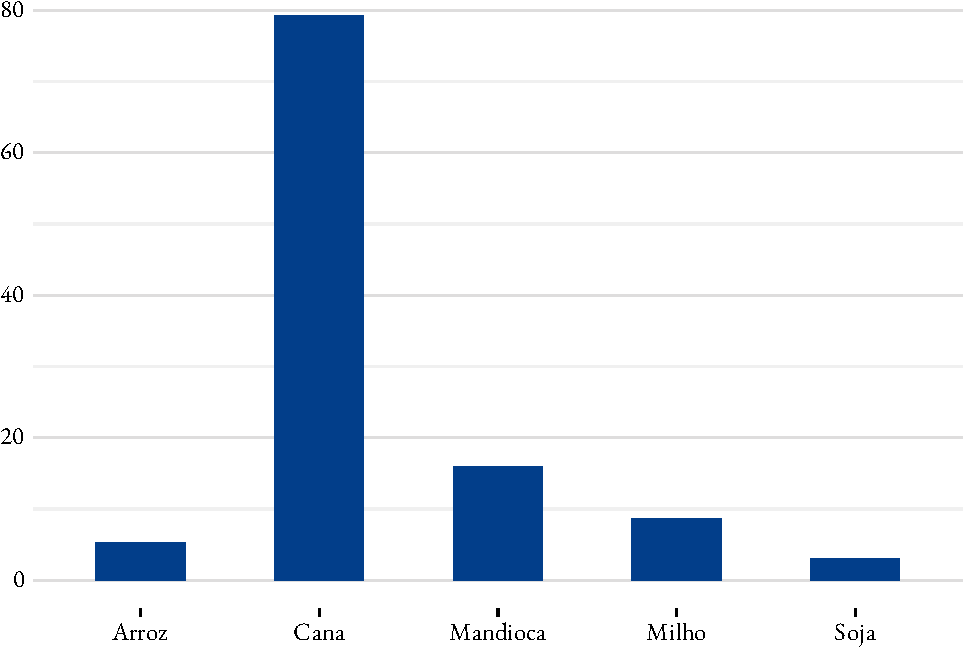
\includegraphics{fig/rendim_medio-1.pdf}
		\source{\acrshort{sidra}/\acrshort{ibge}}
		\label{fig:rendimento}
	\end{subfigure}
	\begin{subfigure}{\linewidth}
		\caption{Área plantada das lavouras}
		\subcap{Em mil hectares. Estimativa anual de setembro}
		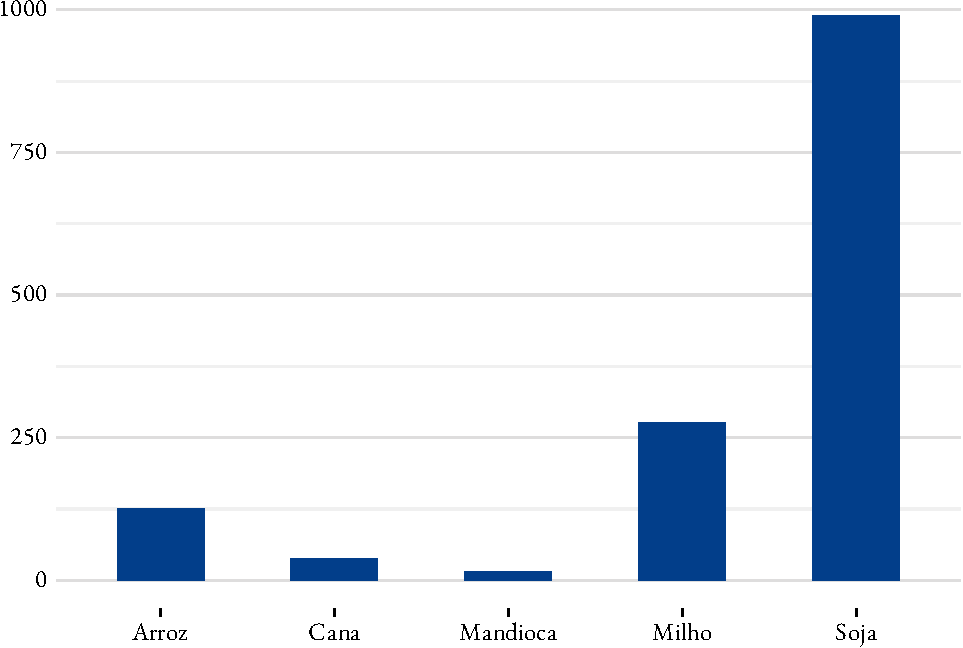
\includegraphics{fig/area_plantada-1.pdf}
		\source{\acrshort{sidra}/\acrshort{ibge}}
		\label{fig:areaplantada}
	\end{subfigure}
\end{figure}

% \section{Rendimento Médio}
\par Dentre os cinco principais produtos cultivados na agricultura tocantinense, o rendimento médio demonstrado na figura \ref{fig:rendimento} mostra como as características próprias de cada um deles tem resultado determinante no cálculo da área que deve ser plantada, visando a quantidade em que será colhida. O cálculo é feito pela divisão entre quilogramas colhidos pela área plantada, significando que, quanto maior o valor do rendimento médio, menor é a área necessária para sua colheita. Sendo assim, os dados mostram que o maior rendimento médio entre estes produtos é da cana-de-açúcar, chegando ao elevado valor de 70,7\%. O segundo produto é a mandioca, com um rendimento médio de 14,3\%, seguido pelo milho, ao total de 7.7\%, arroz, com 4,7\% e por fim, a soja, com um rendimento médio de 2,6\%, ou seja, precisando então de uma vasta área plantada para colher sua quantidade desejada.

% \section{Áreas plantadas e colhidas}

\par Baseando-se no primeiro semestre tem-se os dados das áreas plantadas e colhidas, apresentado na Figura \ref{fig:areaplantada} e consequentemente, os cereais e oleaginosas que mais usam o espaço tocantinense para a produção. No primeiro semestre de 2020, o Tocantins utilizou-se de 1.427.342 hectares para plantação. O maior espaço disso é para a Soja que utilizou-se de 975.513 hectares para a produção, demonstrando que a soja utiliza-se de uma grande quantidade de hectares para a sua produção. Então, a soja tem 68.7\% de utilização do espaço de plantio, em seguida vem o milho que utiliza 18.8\% do território, os dois espaços mais usado para a plantação. O arroz corresponde 8.8\%, em seguida cana com 2.7\% e mandioca com 1\%.

% \section{Produção de leite}
\par O estado tocantinense é conhecido pela sua produção agropecuária e os seus derivados. A fabricação de leite em solo tocantinense no ano de 2019 foi de 132.237 (mil litros), apesar de uma produção grande, o estado ainda não se tornou referência no segmento ficando com menos de 1 percentual na produção do Brasil. O estado mantém valores constantes na sua produção, e não apresenta grande variação nos últimos cinco trimestres. Por fim, sua produção no primeiro trimestre do ano de 2020 teve uma produção de 37.273 (mil litros), apresentando um aumento pequeno comparado ao valor do quarto semestre de 2019 que teve uma produção de 36.369 (mil litros).


% \section{Abate de animais}

\par No quarto trimestre de 2019 os frigoríficos suspenderam abate no Tocantins após o governo cortar incentivos fiscais. Os pecuaristas e empresários do setor sentiram o impacto após o corte do benefício, que era a isenção do imposto sobre circulação de mercadorias e serviços (\acrshort{icms}) para o setor. A alíquota passou a ser de 12\% foi uma das consequências que fez subir o preço da carne para esse ano de 2020.

\begin{smbox}[label={labelbox},nameref={Agricultura}]{Produção em evidência e Agronegócio em geral}
	O Estado tocantinense tem uma economia pautada no agronegócio (não apenas a do Tocantins, a brasileira em si) e com as frequentes desvalorizações cambiais tornou-se atrativo produzir uma commodity como a Soja. O câmbio e a qualidade do solo justificam o desejo de se produzir soja no  estado do Tocantins. O argumento da riqueza gerada pela soja pode ser visto na sessão em que é apresentado os balanços de pagamentos estaduais, e o valor que esse produto gera ao estado.
\\
	No Brasil existem inúmeros órgãos que cuidam e divulgam dados sobre agricultura, sejam municipais, estaduais ou federativo. Uma referencia impar destes dados é o \acrshort{sidra} (Sistema IBGE de Recuperação Automática). Outra referência para agricultura é o \acrshort{ipea} (Instituto de Pesquisa Econômica Aplicada), além das secretarias estaduais e municipais que realizam pesquisas próprias, no estado tocantinense a \acrshort{fieto} e a secretaria da fazenda realizam pesquisas similares.
\end{smbox}

\par É apresentado no abate de animais uma queda no quarto trimestre de 2019, conforme a figura \ref{fig:abate} que foi acarretada pela isenção do incentivo fiscais para o abate dos animais no frigorífico no Tocantins.

\par Enquanto alguns setores da economia são prejudicados pela crise econômica atual, gerada pelo COVID-19. O setor do Agro se reinventa e expande sua produção em frangos, a empresa Grupo goiano SSA Alimentos, dona das marcas “SuperFrango” e “Boua”, esteve no estado no ano de 2019 para conhecer incentivos que o estado oferece para esse setor. A empresa mantém uma distribuidora em Paraíso do Tocantins, mas tem interesse em instalar um complexo industrial para abate de frangos no Estado devido aos incentivos do estado serem bons. Esses incentivos fizeram com que o abate de frangos tenham aumentado no estado, como é demonstrado pela Figura \ref{fig:abate}

% \section{Abate de frangos, bovinos, vacas e novilhas}

\par Já nesse setor de animais, será exposto dados referentes aos abates dessas categorias.

\begin{figure}[!h]
	\caption{Abate dos principais animais}
	\subcap{Mil cabeças}
	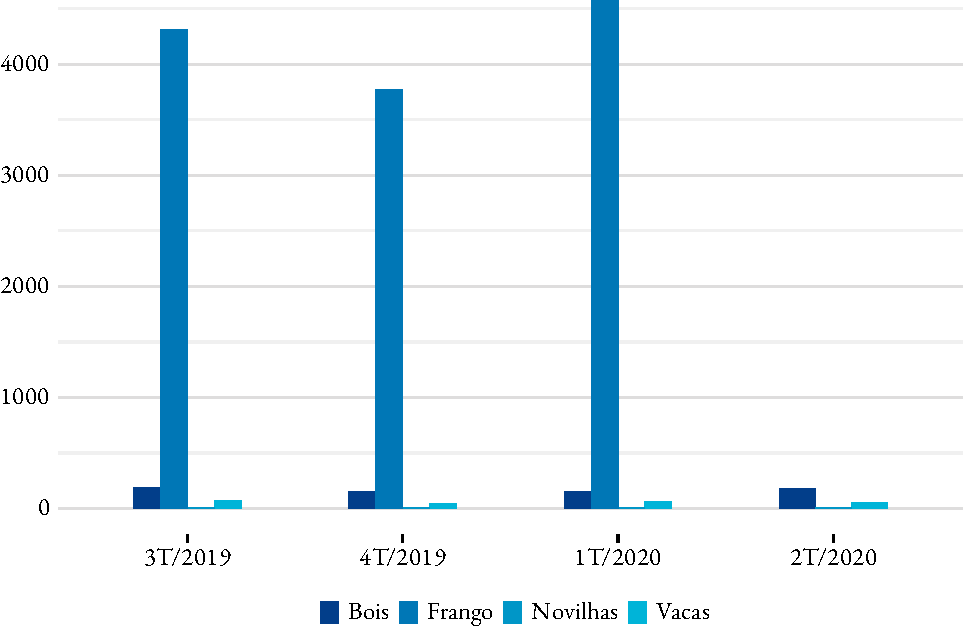
\includegraphics{fig/abates-1.pdf}
	\source{\acrshort{sidra}/\acrshort{ibge}}
	\label{fig:abate}
	\notes{\trimestres}
\end{figure}
